\chapter{Schémas aux différences}

\section{Opérateurs aux différences en dimension 1}

\subsection{Notations}
\label{sec:notation_1D}

On considère $\Omega = [a,b]$, $a<b$, un intervalle de $\mathbb{R}$ de longueur $L=b-a$. Nous utilisons les lettres latines pour noter les fonctions continues : $f(x)$, $u(x)$, ... $x \in \Omega$. Pour $u$ et $v$, des fonctions définies sur $\Omega$, le produit scalaire dans $L^2 ( \Omega )$ est défini par
\begin{equation}
(u,v) = \gint_{\Omega} u(x) \bar{v}(x) dx = \gint_{a}^b u(x) \bar{v}(x) dx.
\end{equation}
Pour $u$ et $v$ à valeurs réelles, on a
\begin{equation}
(u,v) = \gint_{a}^b u(x) v(x) dx.
\end{equation}
La norme sur $L^2(\Omega)$ est donnée par :
\begin{equation}
\| u \|_{L^2(\Omega)} = \sqrt{(u,u)}
\end{equation}
Pour $u \in L^{\infty}(\Omega)$, on note
\begin{equation}
\| u \|_{\infty} = \sup_{x\in\Omega} |u(x)|.
\end{equation}
Une fonction $u : x \in \mathbb{R} \mapsto u(x) \in \mathbb{R}$ est \textit{périodique} de période $L$ si 
\begin{equation}
u(x+L) = u(x) \text{, } \forall x \in \mathbb{R}.
\end{equation}
En particulier, on a $u(a)=u(b)$.

On considère une grille régulière sur $\Omega$ constituée de $N \geq 1$ points :
\begin{equation}
a=x_0 < x_1 < \ldots < x_{N-1} < x_N = b,
\end{equation}
où les valeurs $x_i$ sont définies par :
\begin{equation}
x_i = a + ih\text{, } i = 0,1, \ldots,N \text{ et } h = \dfrac{b-a}{N} \text{ le pas d'espace}. 
\end{equation}

\begin{figure}[htbp]
\begin{center}
\begin{tikzpicture}[scale=1.8]
	\draw [>=stealth, <->] (-2,0.2) -- (-1,.2) ;
	\draw (-1.5,.3) node[above] {$h$} ;
	\draw (-3,0) -- (3,0) ;
	\draw (-3,0) node {$\times$} ;
	\draw (-3,-.2) node[below] {$x_0=a$} ;
	\draw (-2,0) node {$\bullet$} ;
	\draw (-2,-.2) node[below] {$x_1$} ;
	\draw (-1,0) node {$\bullet$} ;
	\draw (-1,-.2) node[below] {$x_2$} ;
	\draw (0,-.2) node[below] {$\ldots$} ;
	\draw (1,0) node {$\bullet$} ;
	\draw (1,-.2) node[below] {$x_{N-2}$} ;
	\draw (2,0) node {$\bullet$} ;
	\draw (2,-.2) node[below] {$x_{N-1}$} ;
	\draw (3,0) node {$\times$} ;
	\draw (3,-.2) node[below] {$x_N =b$} ;
\end{tikzpicture}
\end{center}
\caption{Grille en dimension 1. Les symboles $\times$ désignent les points de bords, les symboles $\bullet$ désignent les points intérieurs de la grille.}
\label{fig:maillage1D}
\end{figure}

Les points $x_0=a$ et $x_N = a + L = b$ sont les points de bord du domaine et les points $(x_j)_{1 \leq j \leq N-1}$ désignent les points intérieurs. 

Nous distinguons trois types de données aux points de grille $x_j$, $0 \leq j \leq N$ :
\begin{enumerate}
\item Une \textit{fonction de grille} est une fonction définie uniquement aux points $(x_j)_{0 \leq j \leq N}$. Les fonctions de grilles sont notées en fonte gothique : $\mathfrak{u}$, $\mathfrak{v}$, ... 
On note
\begin{equation}
\mathfrak{u} = (\mathfrak{u}(x_0), \mathfrak{u}(x_1), \mathfrak{u}(x_2), ... , \mathfrak{u}(x_N)).
\end{equation}
De plus, $l^2_h$ désigne l'espace des fonctions de grille, $h>0$ fixé.
On munit cet espace du produit scalaire et de la norme associée :
\begin{equation}
(\mathfrak{u},\mathfrak{v})_h = h \gsum_{j=0}^N \mathfrak{u}(x_j) \mathfrak{v}(x_j) \text{,  } |\mathfrak{u}|_h^2 = h \gsum_{j=0}^N \mathfrak{u}(x_j)^2.
\end{equation}
On définit aussi la norme infinie pour les fonctions de grille :
\begin{equation}
\| \mathfrak{u} \|_{\infty} = \max_{0\leq j \leq N} |\mathfrak{u}(x_j)|.
\end{equation}
On notera 
\begin{equation}
\mathfrak{u}_j = \mathfrak{u}(x_j) \text{ pour tout } 0\leq j \leq N.  
\end{equation}

On note $l^2_{h,per}$ l'espace des fonctions de grilles périodiques. Si $\mathfrak{u} \in l^2_{h,per}$ alors $\mathfrak{u}(x_0) = \mathfrak{u}(x_N)$ et on a
\begin{equation}
\mathfrak{u}=(\mathfrak{u}(x_0), \mathfrak{u}(x_1), ..., \mathfrak{u}(x_{N-1})).
\end{equation}
Le produit scalaire et la norme associée dans $l^2_{h,per}$ sont
\begin{equation}
(\mathfrak{u},\mathfrak{v})_{h,per} = h \gsum_{j=0}^{N-1} \mathfrak{u}(x_j) \bar{\mathfrak{v}}(x_j) \text{,  } |\mathfrak{u}|_h^2 = h \gsum_{j=1}^N |\mathfrak{u}(x_j)|^2 \text{ avec} \mathfrak{u}, \mathfrak{v} \in l^2_{h,per}.
\end{equation}
La norme infinie dans $l^2_{h,per}$ est
\begin{equation}
\| \mathfrak{u} \|_{\infty} = \max_{0\leq j \leq N-1} |\mathfrak{u}(x_j)|.
\end{equation}



\item Les lettres latines capitales désignent les vecteurs de $\mathbb{R}^{N+1}$ et les matrices de $\mathbb{M}_{N+1}(\mathbb{R})$. Par exemple, soit le vecteur $U \in \mathbb{R}^{N+1}$ des composantes de $\mathfrak{u} \in l^2_h$ :
\begin{equation}
U = \begin{bmatrix}
\mathfrak{u}_0 \\ \mathfrak{u}_1 \\ \vdots \\ \mathfrak{u}_N
\end{bmatrix} =
\begin{bmatrix}
\mathfrak{u}(x_0) \\ \mathfrak{u}(x_1) \\ \vdots \\ \mathfrak{u}(x_N)
\end{bmatrix}
\end{equation}
La norme euclidienne sur $\mathbb{R}^{N+1}$ est notée $|U|$. Elle induit une norme pour les matrices $A \in \mathbb{M}_{N+1}(\mathbb{R})$ définie par
\begin{equation}
|A|_2 = \sup_{U \neq 0} \dfrac{|AU|}{|U|}.
\end{equation}
Si $A$ est symétrique alors :
\begin{equation}
|A|_2 = \rho(A) := \max \left\lbrace |\lambda| \text{ tels que } \lambda \in \Sp (A) \right\rbrace.
\end{equation}
$\rho(A)$ est nommé \textit{rayon spectrale} de $A$.
La norme infinie de $U$ est donnée par :
\begin{equation}
|U|_{\infty} = \max_{1 \leq j \leq N+1} |U_j|.
\end{equation}
La norme sur $\mathbb{M}_{N+1}(\mathbb{R})$ subordonnée à $|\cdot|_{\infty}$ est
\begin{equation}
|A|_{\infty} = \sup_{U \neq 0} \dfrac{|AU|_{\infty}}{|U|_{\infty}} = \max_{1 \leq i \leq N+1} \gsum_{j=1}^{N+1} |A_{i,j}|.
\end{equation}



\item Soit $u: x \in \Omega \mapsto u(x)$, on définit la \textit{fonction de grille} $u^*$ associée à $u$ par :
\begin{equation}
u^*_j = u^*(x_j) \text{ pour } 0 \leq j \leq N.
\end{equation}
$u^*$ est donc la restriction de $u$ aux points de la grille. Si $u$ est une fonction périodique, alors $u^*$ est définit par
\begin{equation}
u^*_j = u^*(x_j) \text{ pour } 1 \leq j \leq N.
\end{equation}
\end{enumerate}

Nous distinguons $l^2_h$, l'espace des fonctions de grilles, de $\mathbb{R}^{N+1}$ même si ces deux espaces sont isomorphes.

Cette distinction permet de faire une claire différences entre :
\begin{itemize}
\item les opérateurs aux différences finies, qui agissent sur les fonctions de grilles,
\item les matrices, qui agissent sur les vecteurs.
\end{itemize}
Les fonctions de grilles contiennent toutes les échelles nécessaires dans le contexte physique alors que les vecteurs sont sans dimension. De plus, le raisonnement au niveau discret est plus naturel avec les fonctions de grilles. Il s'effectue d'une façon abstraite à l'aide d'opérateurs aux différences. En revanche, le codage est effectuée dans le cadre de l'algèbre linéaire.

Si $u : x \in \Omega \mapsto u(x) \in \mathbb{R}$est une fonction régulière telle que $u(a) = u(b) = 0$ alors $(\partial_x u)^*$ désigne la restriction à la grille de la fonction $\partial_x u$ associée à la dérivée première de $u$. On peut approcher cette donnée à l'aide de $\mathfrak{u}_x$ obtenue grâce à l'opérateur $\delta_x$ agissant sur les fonctions de grilles et donné par
\begin{equation}
\mathfrak{u}_{x,j} = \delta_x u^*(x_j) = \dfrac{u(x_{j+1}) - u(x_{j-1})}{2h}.
\end{equation}
En effet, par développement de Taylor, on a 
\begin{equation}
u(x_j+h) = u(x_j) + h \partial_x u(x_j) + \dfrac{h^2}{2} \partial_x^2 u(x_j) + \dfrac{h^3}{6} \partial_x^3 u(\xi) \text{ avec } \xi \in [x_j, x_j+h].
\end{equation}
De la même manière, en $x_j-h$, on a 
\begin{equation}
u(x_j-h) = u(x_j) - h \partial_x u(x_j) + \dfrac{h^2}{2} \partial_x^2 u(x_j) - \dfrac{h^3}{6} \partial_x^3 u(\eta) \text{ avec } \eta \in [x_j-h, x_j].
\end{equation}
Soit $0 \leq j \leq N$, alors
\begin{align*}
\delta_x u^*(x_j) & = \dfrac{u(x_{j+1}) - u(x_{j-1})}{2h}\\
                  & = \dfrac{1}{2h} \left[ 2h \partial_x u(x_j) + \dfrac{h^3}{6} \partial_x^3 u(\xi) + \dfrac{h^3}{6} \partial_x^3 u(\eta) \right]\\
                  & = \partial_x u(x_j) + \dfrac{h^2}{2} \left[ \dfrac{1}{6} \partial_x^3 u(\xi) + \dfrac{1}{6} \partial_x^3 u(\eta) \right] \\
                  & = \partial_x u(x_j) + \dfrac{h^2}{6} \partial_x^3 u(\gamma) \text{ avec } \gamma \in ]x_j-h , x_j+h[ \text{ par théorème des valeurs intermédiaires.}
\end{align*}
L'erreur de troncature est une fonction de grille définie en chaque point du $x_j$ par
\begin{align*}
\mathfrak{t}(x_j) & = \delta_x u^*(x_j) - \delta_x u^*(x_j)\\
                  & = \dfrac{h^2}{6} \partial_x^3 u(\gamma) \text{ avec } \gamma \in ]x_j-h , x_j+h[.
\end{align*}




















\subsection{Transformée de Fourier discrète}

Pour simplifier les notations, on considère $a=0$ et $b=L$. Le pas du maillage est $h = \frac{L}{N}$.
Soit, pour tout $k$ vérifiant $-N/2+1 \leq k \leq N/2$, la fonction $u^k : x \mapsto u^k(x) \in \mathbb{C}$ périodique de période $L$ définie par 
\begin{equation}
u^k(x) = \dfrac{1}{\sqrt{L}} \exp \left( i x \dfrac{2 \pi}{L} \right)
\end{equation}
On définit les \textit{fonctions de base} $\mathfrak{u}^k$ de $l^2_{h,per}$ par
\begin{equation}
\mathfrak{u}^k = \sqrt{h} (u^k)^*
\end{equation}
donc 
\begin{equation}
\mathfrak{u}^k_j = \sqrt{h}  u^k(x_j) = \dfrac{1}{\sqrt{N}} \exp \left( i j k \dfrac{2 \pi}{N} \right) \text{ avec } 0 \leq j \leq N-1.
\label{eq:base_fourier_disc}
\end{equation}


\begin{proposition}
Les fonctions $(\mathfrak{u}^k)_{-N/2+1 \leq k \leq N/2}$ forment une base de $l^2_{h,per}$.
\end{proposition}

\begin{proof}
Soient $k$ et $k'$ sont deux entiers distincts tels que $-N/2+1 \leq k, k' \leq N/2$. $\mathfrak{u}^k, \mathfrak{u}^{k'} \in l^2_{h,per}$ et
\begin{align*}
(\mathfrak{u}^k, \mathfrak{u}^{k'})_{h,per} & = \dfrac{1}{N} \gsum_{j=0}^{N-1} \exp \left( i j k \dfrac{2 \pi}{N} \right) \exp \left( -i j k' \dfrac{2 \pi}{N} \right) \\
		& = \dfrac{1}{N} \gsum_{j=0}^{N-1} \exp \left( i j (k-k') \dfrac{2 \pi}{N} \right)\\
		& = \dfrac{1}{N} \dfrac{1 - \exp \left( i 2 \pi (k-k') \right)}{1 - \exp \left( i (k-k') \dfrac{2 \pi}{N}  \right)} \\
		& = 0
\end{align*}
De plus, si $k=k'$, on a :
\begin{align*}
(\mathfrak{u}^k, \mathfrak{u}^{k})_{h,per} & = \dfrac{1}{N} \gsum_{j=0}^{N-1} \exp \left( i j k \dfrac{2 \pi}{N} \right) \exp \left( -i j k \dfrac{2 \pi}{N} \right) \\
		& = \dfrac{1}{N} \gsum_{j=0}^{N-1} 1 \\
		& = 1.
\end{align*}
\end{proof}

Alors pour tout $\mathfrak{v} \in l^2_{h,per}$ il existe $(\hat{\mathfrak{v}}_k )_{-N/2 \leq k \leq N/2}$ tels que 
\begin{equation}
\mathfrak{v} = \gsum_{-N/2+1}^{N/2} \hat{\mathfrak{v}}_k \mathfrak{u}^k
\end{equation}
En effectuant un produit scalaire par $\mathfrak{u}^{k'}$ un vecteur de base, on obtient
\begin{align*}
(\mathfrak{v}, \mathfrak{u}^{k'})_{h,per} & = \gsum_{k=-N/2+1}^{N/2} \hat{\mathfrak{v}}^k (\mathfrak{u}^k, \mathfrak{u}^{k'})_{h,per} \\
		& = \hat{\mathfrak{v}}_{k'}
\end{align*}
Ainsi, les coefficients $\hat{\mathfrak{v}}_{k} \in \mathbb{C}$ sont donnés par
\begin{equation}
\hat{\mathfrak{v}}_{k} = (\mathfrak{v}, \mathfrak{u}^{k})_{h,per}.
\end{equation}

La donnée $(\hat{\mathfrak{v}}_{k})_{-N/2+1 \leq k \leq N/2} \in \mathbb{C}^N$ est la \textit{transformée de Fourier discrète} de $\mathfrak{v}$. La transformée de Fourier discrète vérifie la formule de Parseval.

\begin{proposition}
\textbf{(Relation de Parseval discrète)} 
Pour tout $\mathfrak{v} \in l^2_{h,per}$, on a 
\begin{equation}
|\mathfrak{v}|_{h,per} = L \gsum_{k=-N/2+1}^{N/2} |\hat{\mathfrak{v}}_k|^2
\end{equation}
\end{proposition}

\begin{proof}
On vérifie la relation par le calcul suivant :
\begin{align*}
|\mathfrak{v}|_{h,per} & = h \gsum_{j=0}^{N-1} \mathfrak{v}_j \bar{\mathfrak{v}_j} \\
	& = h \gsum_{j=0}^{N-1} \gsum_{k=-N/2+1}^{N/2} |\hat{\mathfrak{v}}_k|^2 \underbrace{|\bar{\mathfrak{u}}_j^k|^2}_{=1}\\
	& = h N \gsum_{k=-N/2+1}^{N/2} |\hat{\mathfrak{v}}_k|^2 \\
	& = L \gsum_{k=-N/2+1}^{N/2} |\hat{\mathfrak{v}}_k|^2
\end{align*}
\end{proof}















\subsection{Opérateur de translation périodique}
On se donne $\mathfrak{u} \in l^2_{h,per}$ une fonction de grille périodique.
\begin{definition}
L'opérateur $\tau_p$, $p \in \mathbb{Z}$, est définit, pour $\mathfrak{u}$ une fonction de grille périodique, pour tout $1 \leq j \leq N$ par
\begin{equation}
(\tau_p \mathfrak{u})_j = \mathfrak{u}_{j+p}.
\end{equation}
\end{definition}
L'opérateur linéaire $\tau_p$ agit sur les fonctions périodiques $u : \mathbb{R} \mapsto u(x) \in \mathbb{R}$ par :
\begin{equation}
\tau_p u(x_j) = (\tau_p u^*)_j = u^*_{j+p} = u(x_{j+p}).
\end{equation}
En particulier, lorsque $p=1$, on note $\tau$ l'\textit{opérateur de translation à droite} :
\begin{equation}
\tau = \tau_{1}
\end{equation}
de plus, il est clair que l'on a
\begin{equation}
\begin{array}{rcl}
\tau^0 & = & id\\
\tau^p & = & \underbrace{\tau \circ \tau \circ \tau \circ \cdots \circ \tau}_{p \text{ fois.}}
\end{array}
\end{equation}
L'égalité suivante est vérifiée :
\begin{equation}
\tau^p = \tau_p
\end{equation}
En particulier, on a $\tau^N = \tau_N = id$, donc $\tau$ est inversible et
\begin{equation}
\tau^{-1} = \tau^{N-1}.
\end{equation}
L'analyse des opérateurs périodiques repose sur la diagonalisation de $\tau$. C'est l'objet de la proposition suivante.

\begin{proposition}
les valeurs propres de $\tau$ sont les racines de l'unité $\omega^k \in \mathbb{C}$ avec
\begin{equation}
\omega = \exp \left[ i \dfrac{2 \pi}{N} \right].
\end{equation}

Chaque valeur propre $\omega^k$ est associée à une fonction propre $\mathfrak{u}^k \in l^2_{h,per}$, avec $-\frac{N}{2}+1 \leq k \leq \frac{N}{2}$, données par la proposition \ref{eq:base_fourier_disc}.
\label{prop:eigenvaluevector_tau}
\end{proposition}

\begin{proof}
Soit $j$ et $k$ tels que $1 \leq j \leq N$ et $-\frac{N}{2}+1 \leq k \leq \frac{N}{2}$. Alors
\begin{equation}
(\tau \mathfrak{u}^k)_j = \mathfrak{u}^k_{j+1}  = \dfrac{1}{\sqrt{N}}\exp \left[ i (j+1) \dfrac{2 \pi k}{N} \right] = \dfrac{1}{\sqrt{N}} \exp \left[ i j \dfrac{2 \pi k}{N} \right] \exp \left[ i \dfrac{2 \pi k}{N} \right]  = \omega^k \mathfrak{u}_j^k
\end{equation}
d'où le résultat.
\end{proof}
Connaissant les valeurs et fonctions propres de $\tau$, on déduit en déduit la diagonalisation de $\tau$.

\begin{corollaire}
L'opérateur $\tau$ est diagonalisable et 
\begin{equation}
\tau = \gsum_{k = -N/2+1}^{N/2} \omega^k \mathfrak{u}^k
\end{equation}
où les fonctions propres $\mathfrak{u}^k$ et les valeurs propres $\omega^k$ sont données dans la proposition \ref{prop:eigenvaluevector_tau}
\end{corollaire}
Soit $P \in \mathbb{C}[X]$ un polynôme alors les valeurs propres et fonctions propres de $P(\tau)$ sont connues.

\begin{proposition}
Les fonctions propres de $P(\tau)$ sont les fonctions de grilles $\mathfrak{u}^k$.
Chaque fonction propre est associé à la valeur propre $P(\omega^k)$ avec $-N/2+1 \leq k \leq N/2$.
\label{prop:eigen_tau}
\end{proposition}

\begin{proof}
$P$ est un polynôme de $\mathbb{C}[X]$ donc il existe un nombre finis d'éléments de $\mathbb{C}$ notés $a_0$, $a_1$, $a_2$, ... tels que
\begin{equation}
P(X) = \gsum_{n=0} a_n X^n.
\end{equation}
Soient $j$ et $k$ tels que $1 \leq j \leq N$ et $-N/2+1 \leq k \leq N/2$, alors 
\begin{equation}
(P(\tau) \mathfrak{u}^k)_j = \left( \gsum_{n=0} a_n \tau_n \mathfrak{u}^k \right)_j = \gsum_{n=0} a_n \mathfrak{u}^k_{j+n}  = \gsum_{n=0} a_n (\omega^k)^n \mathfrak{u}^k_j = P(\omega^k) \mathfrak{u}^k_j
\end{equation}
d'où le résultat.
\end{proof}

Notons que cette proposition est vraie pour tout opérateur diagonalisable à la place de $\tau$.

L'opérateur de translation $\tau$ agit sur les fonctions de grilles $\mathfrak{u}$. Il est associé à $T \in \mathbb{M}_N \left( \mathbb{R} \right)$ la matrice agissant sur les vecteurs $U$ de $\mathbb{R}^N$.
On définit $\vec_1$ l'opérateur transformant un élément de $l_{h,per}^2$ en un vecteur de $\mathbb{R}^N$ :

\begin{definition}
Soient $\mathfrak{u} \in l^2_{h,per}$ une fonction de grille et $(\mathbf{e}_j)_{1 \leq j \leq N}$ la base canonique de $\mathbb{R}^N$. On définit l'opérateur $\vec_1$ par :
\begin{equation}
\begin{array}{rcl}
\vec_1 : l^2_{h,per} & \rightarrow & \mathbb{R}^N\\
         \mathfrak{u} & \mapsto & \vec_1 ( \mathfrak{u} ) 
\end{array}
\end{equation}
avec 
\begin{equation}
\vec_1 ( \mathfrak{u} ) =\gsum_{j=1}^N \mathfrak{u}_{j-1} \mathbf{e}_j.
\end{equation}
\end{definition}

Il s'agit d'un opérateur transformant directement une fonction de grille $\mathfrak{u} \in l^2_{h,per}$ en un vecteur $U$ de $\mathbb{R}^N$ 
\begin{equation}
U = \vec_1( \mathfrak{u} ) = \begin{bmatrix}
\mathfrak{u}_0\\
\mathfrak{u}_1\\
\vdots\\
\mathfrak{u}_{N-1}\\
\end{bmatrix}
\end{equation}
La matrice $T$ est donnée par

\begin{equation}
T = \begin{bmatrix}
0 & 1 &   &   &   \\ 
  & 0 & 1 & (0) &   \\ 
  &   & \ddots & \ddots &   \\ 
  & (0) &   & 0 & 1 \\ 
1 &   &   &   & 0
\end{bmatrix} 
\end{equation}

La matrice $T$ agit sur un vecteur $U = \begin{bmatrix}
U_0 & U_0 & \cdots & U_{N-1} 
\end{bmatrix}^T \in \mathbb{R}^N $ de telle manière que, pour tout $1 \leq j \leq N$, on a 
\begin{equation}
(TU)_j = U_{j+1}
\end{equation}
C'est à dire
\begin{equation}
\vec_1 ( \tau \mathfrak{u} ) = T \vec_1 ( \mathfrak{u} ). 
\end{equation}
Les propriétés concernant les valeurs propres de $\tau$ sont aussi vérifiées par $T$.

\begin{corollaire}
\begin{itemize}
\item Les valeurs propres de $T$ sont les valeurs $(\omega^k)_{-N/2+1 \leq k \leq N/2}$. 
Chaque valeur propre est associée à un vecteur propre $U^k$ vérifiant :
\begin{equation}
U^k = \vec_1 (\mathfrak{u}^k )
\label{eq:eigenvectorT}
\end{equation}
où $\mathfrak{u}^k$ et $\omega$ sont données dans la proposition \ref{prop:eigenvaluevector_tau}.

\item Si $P \in \mathbb{R}_{N-1}[X]$ alors les valeurs propres de $P(T)$ sont 
\begin{equation}
P(\omega^k)
\end{equation}
chaque valeur propre $P(\omega^k)$ de $T$ est associée au vecteur propre $\vec_1 (\mathfrak{u}^k )$.
\end{itemize}
\label{prop:eigen_P(tau)}
\end{corollaire}

Les vecteurs propres de $T$ forment une base orthonormée de $\mathbb{R}^N$ pour le produit scalaire usuel.



















\subsection{Opérateurs aux différences discrets}

Soit $\mathcal{L}$ un opérateur différentiel. On s'intéresse ici à approcher cet opérateur par $L_h$ et à estimer l'erreur commise via cette approximation.

\begin{definition}
Le couple $(L_h, R_h)$ est consistant avec $L$ à l'ordre $\alpha$ si pour tout $u : \mathbf{x} \in \mathbb{R} \mapsto u(\mathbf{x}) \in \mathbb{R}$ régulière et périodique alors 
\begin{equation}
L_h u^* - R_h (\mathcal{L}(u)^*) = \mathcal{O} \left ( h^{\alpha} \right)
\end{equation}
avec $R_h$ un opérateur d'interpolation et $L_h$ un opérateur d'approximation de $\mathcal{L}$.
\end{definition}





Introduisons l'\textit{opérateurs aux différences centré} usuel
\begin{equation}
\delta_x = \dfrac{\tau_1 - \tau_{-1}}{2h}
\end{equation}
Appliqué à la fonction de grille $\mathfrak{u}$, cet opérateur vérifie 
\begin{equation}
\delta_x \mathfrak{u}_i = \dfrac{\mathfrak{u}_{i+1} - \mathfrak{u}_{i-1}}{2h} \text{ pour } 1 \leq i \leq N.
\end{equation}
Il s'agit d'un opérateur permettant d'approcher la dérivée première au sens où

\begin{proposition}
Soit $u: x \in \Omega \mapsto u(x) \in \mathbb{R}$ et $u^*$ la fonction de grille correspondante. Si $u \in \mathcal{C}^3 (\Omega)$ alors 
\begin{equation}
\delta_x u^*_i - u'(x_i) = \dfrac{h^2}{6} u^{(3)}(\alpha_i) \text{ avec } \alpha_i \in [x_{i-1}, x_{i+1}],
\end{equation}
\end{proposition}

\begin{proof}
Comme $u$ est de classe $\mathcal{C}^3$, on considère les développements de Taylor :
\begin{equation}
u(x_i+h) = u(x_i) + h u'(x_i) + \dfrac{h^2}{2} u''(x_i) + \dfrac{h^3}{6} u^{(3)} (\eta_i) \text{ avec } \eta_i \in [x_i, x_{i+1}]
\end{equation}
et celui en $x-h$ :
\begin{equation}
u(x_i-h) = u(x_i) - h u'(x_i) + \dfrac{h^2}{2} u''(x_i) - \dfrac{h^3}{6}u^{(3)}(\xi_i) \text{ avec } \xi_i \in [x_{i-1}, x_{i}]
\end{equation}
Alors par différence, on retrouve la formule souhaitée : 
\begin{equation}
\delta_x u^*_i = u'(x_i) + \dfrac{h^2}{12} \left[ u^{(3)}(\xi_i) + u^{(3)}(\eta_i) \right]  \text{ avec } \xi_i, \eta_i \in [x_{i-1}, x_{i+1}],
\end{equation}
On conclut grâce au théorème des valeurs intermédiaires.
\end{proof}

Ainsi, $\delta_x$ est un opérateur d'approximation de la dérivée première à l'ordre 2. Il est possible de généraliser ce procéder.
Soit $P \in \mathbb{N}^*$. 
On définit $\delta_{P,x}$ l'opérateur
\begin{equation}
\delta_{2P,x} = \gsum_{j=1}^P a_j \dfrac{\tau_j - \tau_{-j}}{2 j h}
\label{eq:explicite_dx}
\end{equation}
où  pour tout $1 \leq j \leq P$, on a $a_j \in \mathbb{R}$. 




\begin{theoreme}
L'opérateur $\delta_{2P,x}$ est un opérateur d'approximation de la dérivée première à l'ordre $2P$ si et seulement si les coefficients $(a_j)_{1 \leq j \leq P}$ sont solutions de :
\begin{equation}
\left\lbrace
\begin{array}{rcll}
\gsum_{j=1}^P a_j & = & 1 & \\
\gsum_{j=1}^P j^{2k} a_j & = & 0 \text{ pour tous } 1 \leq k \leq P-1.
\end{array}
\right.
\label{eq:syst_opexplicite_P}
\end{equation}
L'erreur de troncature est de la forme :
\begin{equation}
\left(u' \right)_i^* - \delta_{2P,x} u^*_i = h^{2P}\sum_{j=1}^P a_j 2P \dfrac{j^{2P}}{2(2P+1)!} u^{(2P+1)}(\alpha_i) .
\end{equation}
avec $\alpha_i \in [x_{i-P}, x_{i+P}]$.
\label{th:consistance_delta_x_explicite}
\end{theoreme}

\begin{proof}
Soit $u : x \in \Omega \mapsto u(x) \in \mathbb{R}$ une fonction de classe $\mathcal{C}^{2P+1}( \Omega)$ et $u^*$ la fonction de grille correspondante.

On considère les développements de Taylor :
\begin{equation}
\begin{array}{rcl}
u(x_i + jh) & = & u(x_i) + j h u'(x_j) + \cdots + \dfrac{(jh)^k}{k!}u^{(k)}(x_i) + \cdots +\dfrac{(jh)^{2P+1}}{(2P+1)!} u^{(2P+1)}(\xi_j)\\
u(x_i - jh) & = & u(x_i) - j h u'(x_j) + \cdots + \dfrac{(-jh)^k}{k!}u^{(k)}(x_i) + \cdots +\dfrac{(-jh)^{2P+1}}{(2P+1)!} u^{(2P+1)}(\eta_j)
\end{array}
\end{equation}
avec $\xi_j \in [x_i, x_i+jh]$ et $\eta_j \in [x_i-jh, x_i]$. En combinant ces deux égalités, on a
\begin{equation}
\dfrac{\tau_ju^*_i - \tau_{-j} u^*_i}{2jh} = u'(x_i) + \cdots + \dfrac{(jh)^{k-1}(1 - (-1)^k)}{2 \cdot k!} u^{(k)}(x_i) + \cdots +\dfrac{(jh)^{2P}}{2(2P+1)!} \left( u^{(2P+1)}(\xi_j) + u^{(2P+1)}(\eta_j) \right)
\end{equation}
Donc la combinaison linéaire de ces termes pondérée par les coefficients $(a_j)_{1 \leq j \leq P}$ est consistante avec la dérivée première si et seulement si :
\begin{equation}
\left\lbrace
\begin{array}{rcll}
\gsum_{j=1}^P a_j & = & 1 & \\
\gsum_{j=1}^P j^{k-1} \dfrac{(1 - (-1)^k)}{k!} a_j & = & 0 \text{ pour tous } 1 \leq k \leq 2P-1.
\end{array}
\right.
\end{equation}
La seconde égalité est vérifiée pour tout $k$ pair. Ce système se simplifie en :
\begin{equation}
\left\lbrace
\begin{array}{rcll}
\gsum_{j=1}^P a_j & = & 1 & \\
\gsum_{j=1}^P j^{2k} a_j & = & 0 \text{ pour tous } 1 \leq k \leq P-1.
\end{array}
\right.
\end{equation}
L'erreur de troncature prend la forme
\begin{equation}
u'(x_i) - \delta_{2P,x} u^*_i = h^{2P} \sum_{j=1}^P a_j \dfrac{j^{2P}}{2(2P+1)!} \left( u^{(2P+1)}(\xi_j) + u^{(2P+1)}(\eta_j) \right).
\end{equation}
pour conclure, on utilise le théorème des valeurs intermédiaires.
\end{proof}

\begin{proposition}
Le système \eqref{eq:syst_opexplicite_P} admet une unique solution.
\end{proposition}

\begin{proof}
Pour montrer que la solution du système \eqref{eq:syst_opexplicite_P} admet une unique solution, il suffit de montrer que si 
\begin{equation}
A = \begin{bmatrix}
(1^2)^0 & (2^2)^0 & (3^2)^0 & (4^2)^0 & \cdots & (P^2)^0\\
(1^2)^1 & (2^2)^1 & (3^2)^1 & (4^2)^1 & \cdots & (P^2)^1\\
(1^2)^2 & (2^2)^2 & (3^2)^2 & (4^2)^2 & \cdots & (P^2)^2\\
\vdots  &         &         & \vdots  &        &  \vdots\\
(1^2)^{P-1} & (2^2)^{P-1} & (3^2)^{P-1} & (4^2)^{P-1} & \cdots & (P^2)^{P-1}
\end{bmatrix} 
\end{equation}
alors $A$ est inversible.
On remarque que $\det (A)$ est un déterminant de Van Der Monde dont les coefficients sont strictement croissants donc $\det(A) > 0$ et en particulier, $A$ est inversible. La solution de \eqref{eq:syst_opexplicite_P} existe et est unique.
\end{proof}

On suppose à présent les coefficients de $\delta_{P,x}$ issus du système \ref{eq:syst_opexplicite_P}. Il existe $(a_j)_{1 \leq j \leq P}$ tels que 
\begin{equation}
\delta_{2P,x} = \gsum_{j=1}^P a_j \dfrac{\tau_j - \tau_{-j}}{2jh}
\end{equation}
Or, on a déja vu que $\tau^{-1} = \tau_{-1} = \tau^{N-1}$, c'est à dire plus généralement
\begin{equation}
\tau_{-l} = \tau^{-l} = \tau^{N-l} \text{ avec } l \in \mathbb{Z}.
\end{equation}
D'où
\begin{align*}
\delta_{2P,x} & = \gsum_{j=1}^P a_j \dfrac{\tau_j - \tau_{-j}}{2jh}\\
	& = \gsum_{j=1}^P \dfrac{a_j}{2jh} \left( \tau_j - \tau_{-j} \right)\\
	& = \gsum_{j=1}^P \dfrac{a_j}{2jh} \left( \tau^j - \tau^{N-j} \right)\\
	& = \dfrac{1}{h} Q_P(\tau)
\end{align*}
avec $Q_P$ un polynôme de $\mathbb{R}_{N-1}[X]$ donné par
\begin{equation}
Q_{2P}(X) = \gsum_{j=1}^P \dfrac{a_j}{2j} \left( X^j - X^{N-j} \right)
\end{equation}

On en déduit quelques opérateurs d'approximation de la dérivée première.
\begin{corollaire}
Soit $u :  x \in \Omega \mapsto u(x) \in \mathbb{R}$ une fonction donnée. 
\begin{itemize}
\item Si $u \in \mathcal{C}^3 (\Omega)$ alors l'opérateur :
\begin{equation}
\delta_{2,x} = \delta_x = \dfrac{\tau_1 - \tau_{-1}}{2h} = \dfrac{1}{h}Q_2(\tau)
\label{eq:derprem_order2}
\end{equation}
est un opérateur d'approximation de la dérivée première à l'ordre 2 ($P=1$) avec 
\begin{equation}
Q_2(X) = \dfrac{1}{2}(X-X^{N-1}),
\end{equation}
\item Si $u \in \mathcal{C}^5 (\Omega)$ alors l'opérateur :
\begin{equation}
\delta_{4,x} = \dfrac{4}{3} \dfrac{\tau_1 - \tau_{-1}}{2h} - \dfrac{1}{3} \dfrac{\tau_2 - \tau_{-2}}{4h} = \dfrac{1}{h}Q_4(X)
\label{eq:derprem_order4}
\end{equation}
est un opérateur d'approximation de la dérivée première à l'ordre 4 ($P=2$), avec
\begin{equation}
Q_4(X) = \dfrac{2}{3} (X-X^{N-1}) - \dfrac{1}{12} (X^2-X^{N-2})
\end{equation}
\item Si $u \in \mathcal{C}^7 (\Omega)$ alors l'opérateur :
\begin{equation}
\delta_{6,x} = \dfrac{3}{2} \dfrac{\tau_1 - \tau_{-1}}{2h} - \dfrac{3}{5} \dfrac{\tau_2 - \tau_{-2}}{4h} + \dfrac{1}{10} \dfrac{\tau_3 - \tau_{-3}}{6h} = \dfrac{1}{4} Q_6(X)
\label{eq:derprem_order6}
\end{equation}
est un opérateur d'approximation de la dérivée première à l'ordre 6 ($P=3$), avec
\begin{equation}
Q_6(X) = \dfrac{3}{4} (X-X^{N-1}) - \dfrac{3}{20} (X^2-X^{N-2}) + \dfrac{1}{60} (X^3-X^{N-3})
\end{equation}
\item Si $u \in \mathcal{C}^9 (\Omega)$ alors l'opérateur :
\begin{equation}
\delta_{8,x} = \dfrac{8}{5} \dfrac{\tau_1 - \tau_{-1}}{2h} - \dfrac{4}{5} \dfrac{\tau_2 - \tau_{-2}}{4h} + \dfrac{8}{35} \dfrac{\tau_3 - \tau_{-3}}{6h} - \dfrac{1}{35} \dfrac{\tau_4 - \tau_{-4}}{8h} = \dfrac{1}{h}Q_8(X)
\label{eq:derprem_order8}
\end{equation}
est un opérateur d'approximation de la dérivée première à l'ordre 8 ($P=4$), avec
\begin{equation}
Q_8(X) = \dfrac{4}{5} (X-X^{N-1}) - \dfrac{1}{5} (X^2-X^{N-2}) + \dfrac{4}{105} (X^3-X^{N-3}) - \dfrac{1}{180} (X^4-X^{N-4}).
\end{equation}
\end{itemize}
\end{corollaire} 

Les valeurs propres de $\delta_{2P,x}$ sont immédiatement connues grâce à sa forme polynomiale et la proposition \ref{prop:eigen_P(tau)} :
\begin{proposition}
Les valeurs propres de $\delta_{2P,x}$ sont
\begin{equation}
\dfrac{1}{h}Q_{2P}(\omega^k)
\end{equation}
où $\omega^k$ est la k-ième racine de l'unité, avec $-N/2+1 \leq k \leq N/2$, et est associée à la fonction propre $\mathfrak{u}^k$.
\end{proposition}

Soit $-N/2+1 \leq k \leq N/2$. On rappelle que
\begin{equation}
\mathfrak{u}^k = \sqrt{h}(u^k)^* \text{ avec } u^k(x)=\dfrac{1}{\sqrt{L}} \exp \left( i \dfrac{2 \pi x}{L} \right)
\end{equation}
On a alors directement les deux égalités suivantes 
\begin{equation*}
\begin{array}{rcl}
\delta_{2P,x} (u^k)^* & = & \dfrac{1}{h}Q_{2P} (\omega^k) (u^k)^*\\
(\partial_x u^k)^* & = & i \dfrac{2 \pi k}{L} (u^k)^*
\end{array}
\end{equation*}
On considère que l'opérateur $\delta_{2P,x}$ est consistant avec $\partial_x$ à l'ordre $2P$, alors
\begin{align*}
-ih \left( \delta_{2P,x} (u^k)^* - (\partial_x u^k)^* \right) & = \left( -i Q_{2P}(\omega^k) + \dfrac{2 \pi k}{N} \right) \\
	& = \left( -i Q_{2P}\left( \exp(i \theta) \right) + \theta \right) \text{ avec } \theta = \dfrac{2 \pi k}{N}\\
	& = \mathcal{O} \left( h^{2P+1} \right).
\end{align*}
La consistance du schéma assure que $i Q_{2P}\left( \exp(i \theta) \right)$ est proche de $\theta$. En particulier, on remarque que
\begin{equation}
 i Q_{2P}(e^{i0}) = 0 \text{ et }  i Q_{2P}(e^{i \pi}) = 0 \neq \pi
\end{equation}
Ainsi, la fréquence $k=0$ est parfaitement représentée et la fréquence $k = N/2$ est très mal représentée par l'ensemble des schémas aux différences finies considérées.

On sait que $-N/2+1 \leq k \leq N/2$ donc $-\pi \leq \theta \leq \pi$. De plus, la fonction de $\theta$ modifiée : $\theta \mapsto -i Q_{2P}\left( \exp(i \theta) \right)$  est donnée par
\begin{equation}
-i Q_{2P}\left( \exp(i \theta) \right) = \gsum_{j=1}^P a_j \sin(j \theta)
\end{equation}
et est impaire. On peut se contenter de comparer $\theta$ et $-i Q_{2P}\left( \exp(i \theta) \right)$ pour $\theta \in [0 , \pi]$. Le graphique de comparaison est donné dans en Fig. \ref{fig:freq_classic}. On constate que plus le schéma est d'ordre élevé, meilleure est la représentation des hautes fréquences.

\begin{figure}[htbp]
\begin{center}
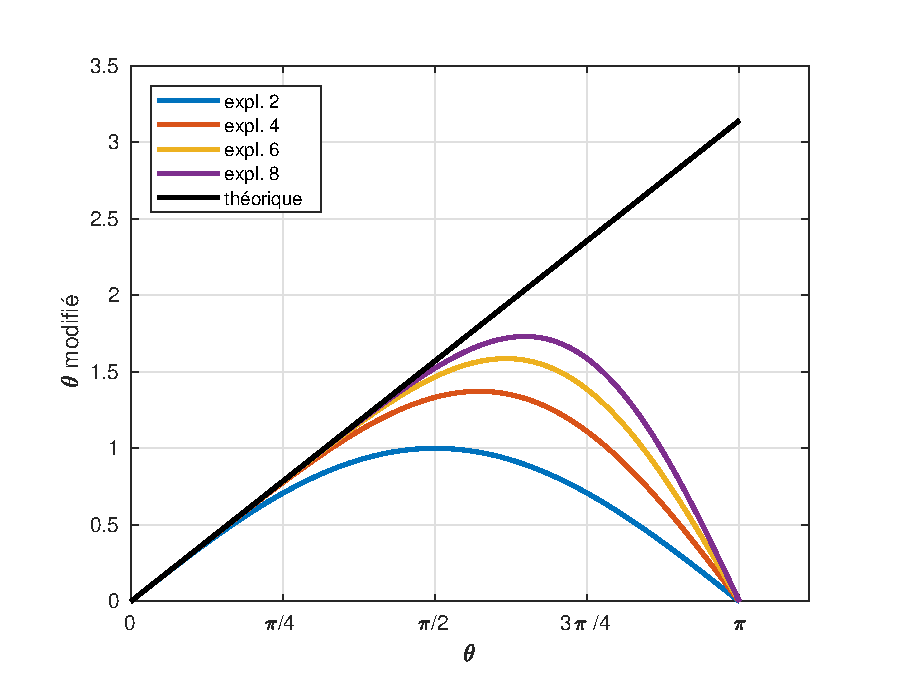
\includegraphics[scale=.6]{freq_classic.eps}
\end{center}
\caption{Représentation de $i Q_{2P}\left( \exp(i \theta) \right)$ en fonction de $\theta$ pour les schémas d'approximation explicites $\delta_{x,P}$ d'ordres 2, 4, 6 et 8.}
\label{fig:freq_classic}
\end{figure}

On définit $D_{2P} \in \mathbb{M}_N(\mathbb{R})$ la matrice associée à l'opérateur $\delta_{2P,x}$ :
\begin{equation}
D_{2P} = \dfrac{1}{h} Q_{2P}(T).
\end{equation}
La relation suivante est alors vérifiée
\begin{equation}
\vec_1(\delta_{2P,x} \mathfrak{u}) = D_{2P} \vec_1 ( \mathfrak{u} )
\end{equation}
pour tout $\mathfrak{u} \in l^2_{h,per}$.

Par exemple, le schéma centré d'ordre 2 $\delta_x = \delta_{2,x}$ est associée à la matrice
\begin{equation}
D_2 = \dfrac{1}{2h}
\begin{bmatrix}
0 & 1 &   &   &   & -1 \\ 
-1 & 0 & 1 &   & (0) &   \\ 
  & -1 & 0 & 1 &   &   \\ 
  &   & \ddots & \ddots & \ddots &   \\ 
  & (0) &   & -1 & 0 & 1 \\ 
1 &   &   &   & -1 & 0
\end{bmatrix} 
\end{equation}

\begin{proposition}
Les valeurs propres de $D_{2P}$ sont données par $\dfrac{1}{h}Q_{2P}(\omega^k)$ avec $-N/2 +1 \leq k \leq N/2$. Chaque valeur propre est associée à un vecteur propre $\vec_1{\mathfrak{u}^k}$.
\end{proposition}

\begin{proposition}
La matrice $D_{2P}$ est antisymétrique.
\end{proposition}

\begin{proof}
Montrons que $D_{2P}^T = - D_{2P}$ :
\begin{align*}
D_{2P}^T & = \dfrac{1}{h} Q_{2P}(T)^T \\
	& = \dfrac{1}{h} \left( \gsum_{j=1}^P \dfrac{a_j}{2j} (T^j - T^{N-j}) \right)^T\\
	& = \dfrac{1}{h}\gsum_{j=1}^P \dfrac{a_j}{2j} ((T^j)^T - (T^{N-j})^T) \\
	& = \dfrac{1}{h}\gsum_{j=1}^P \dfrac{a_j}{2j} (T^{N-j} - T^{j}) \\
	& = - \dfrac{1}{h} \gsum_{j=1}^P \dfrac{a_j}{2j} (T^j - T^{N-j}) \\
	& = - D_{2P}
\end{align*}
d'où le résultat.
\end{proof}





























\subsection{Opérateurs Hermitiens périodiques 1D}

Dans son article \cite{Lele1991}, S. K. Lele présente une méthode permettant d'approcher la dérivée en un point en ajoutant une partie implicite au schéma de la forme \eqref{eq:explicite_dx}. Dans ce chapitre, nous ne considérons que les schémas à 3 points implicites. Définissons l'opérateur $\sigma_{x}$ par :

\begin{equation}
(\sigma_{x} \mathfrak{u})_j = (1-2\beta) \mathfrak{u}_j + \beta \left( \mathfrak{u}_{j+1} + \mathfrak{u}_{j-1} \right)
\end{equation}

\begin{theoreme}
Si les coefficients réels $\beta$ et $(a_i)_{1 \leq i \leq P}$ sont solutions de 
\begin{equation}
\left\lbrace
\begin{array}{rcl}
\gsum_{p=1}^P a_p & = & 1 \\
\gsum_{p=1}^P a_p \dfrac{p^{2n}}{2n+1} & = & 2 \beta  \text{ pour } n=1,2,...P
\end{array}
\right.
\label{eq:hermitian_system}
\end{equation}
et si $u$ est une fonction de $\mathcal{C}^{2P+3}$, alors pour tout $0 \leq i \leq N-1$, on a 
\begin{equation}
(\delta_{2P,x} u^*)_i - (\sigma_{3,x} u'^*)_i = \\
h^{2P+2} \left( \gsum_{p=1}^P a_p  \dfrac{j^{2P+2} P}{(2P+3)!}  - \dfrac{2\beta}{(2P+2)!}   \right)u^{(2P+3)}(\rho)
\label{eq:eq_cons}
\end{equation}
avec $\rho \in [x_{i-P}, x_{i+P}]$.
\end{theoreme}

\begin{proof}
Soit $u : x \in \Omega \mapsto u(x) \in \mathbb{R}$ une fonction de classe $\mathcal{C}^{2P+3}( \Omega)$ et $u^*$ la fonction de grille correspondante.

On considère les développements de Taylor :
\begin{equation}
\begin{array}{rcl}
u(x_i + ph) & = & u(x_i) + p h u'(x_j) + \cdots + \dfrac{(ph)^k}{k!}u^{(k)}(x_i) + \cdots +\dfrac{(ph)^{2P+3}}{(2P+3)!} u^{(2P+3)}(\xi_p)\\
u(x_i - ph) & = & u(x_i) - p h u'(x_j) + \cdots + \dfrac{(-ph)^k}{k!}u^{(k)}(x_i) + \cdots +\dfrac{(-ph)^{2P+3}}{(2P+3)!} u^{(2P+3)}(\eta_p)
\end{array}
\end{equation}
avec $\xi_p \in [x_i, x_i+ph]$ et $\eta_p \in [x_i-ph, x_i]$. En combinant ces deux égalités, on a
\begin{equation}
\dfrac{\tau_pu^*_i - \tau_{-p} u^*_i}{2ph} = u'(x_i) + \cdots + \dfrac{(ph)^{k-1}(1 - (-1)^k)}{2 \cdot k!} u^{(k)}(x_i) + \cdots +\dfrac{(ph)^{2P+2}}{2(2P+3)!} \left( u^{(2P+3)}(\xi_p) + u^{(2P+3)}(\eta_p) \right)
\label{eq:preuve_herm1}
\end{equation}

D'autres part, on a 
\begin{equation}
(1-2\beta) u'^*_i + \beta \left( \tau_1 u'^*_{i} + \tau_{-1} u'^*_{i} \right) = u'^*_i +  \gsum_{k=1}^{2P+1} \beta \dfrac{h^{k}}{k!} \left( 1 + (-1)^k \right) u^{(k+1)}(x_i)+ \beta \dfrac{h^{2P+2}}{(2P+2)!} \left(u^{(2P+3)}(\varrho) + u^{(2P+3)}(\sigma) \right) 
\label{eq:preuve_herm2}
\end{equation}
avec $\varrho \in [x_i, x_i + h]$ et $\sigma \in [x_i, x_i - h]$. 

On remarque directement que \eqref{eq:preuve_herm2} et $\gsum_{p=0}^P a_p  \eqref{eq:preuve_herm1}$ coïncident pour les puissances de $h$ impaires. 

Pour les autres valeurs, l'égalité est vrai si les coefficients $a_p$ et $\beta$ sont solutions de \eqref{eq:hermitian_system}. L'erreur de troncature prend directement la forme 

\begin{multline}
(\delta_{2P,x} u^*)_i - (\sigma_{3,x} u'^*)_i = \\
h^{2P+2} \left( \gsum_{p=1}^P a_p  \dfrac{p^{2P+2}}{2(2P+3)!} \left( u^{(2P+3)}(\xi_j) + u^{(2P+3)}(\eta_j) \right) - \dfrac{\beta}{(2P+2)!} \left(u^{(2P+3)}(\varrho) + u^{(2P+3)}(\sigma) \right) \right)
\end{multline}
On conclut en utilisant le théorème des valeurs intermédiaires.
\end{proof}

\begin{proposition}
Le système \eqref{eq:hermitian_system} admet une unique solution.
\end{proposition}

\begin{proof}
TBA.
\end{proof}

\begin{proposition}
Les valeurs propres de $\sigma_x$ sont
\begin{equation}
R(\omega^k) \text{ avec } R(X) = (1-2 \beta) + \beta(X+X^{N-1}) \text{ et } -N/2+1 \leq k \leq N/2.
\end{equation}
Le vecteur propre associé à $R(\omega^k)$ est $\mathfrak{u}^k$.
\end{proposition}

\begin{proof}
TBA.
\end{proof}

\begin{corollaire}
L'opérateur $\sigma_x$ est inversible si
\begin{equation}
\beta < \dfrac{1}{4}.
\end{equation}
\end{corollaire}

\begin{definition}
On suppose que $\beta$ et $(a_p)_{1 \leq p \leq P}$ sont solutions de \eqref{eq:hermitian_system} et que $\beta < 1/4$, on définit l'\textit{opérateur hermitien} d'approximation de la dérivée première $\delta_x^H$ par 
\begin{equation}
\delta_{2P,x}^H = \sigma_x^{-1} \circ \delta_{2P,x}.
\end{equation}
\end{definition}

\begin{theoreme}
Si $u : x \in \Omega \mapsto u(x) \in \mathbb{R}$ est une fonction de classe $\mathcal{C}^{(2P+3)}$.
Alors 
\begin{equation}
\| u'^* - \delta_{2P,x}^H u^* \|_{\infty} \leq C h^{2P+2} \| u^{(2P+3)} \|_{\infty}
\end{equation}
où $C$ est une constante indépendante de $u$.
\end{theoreme}

\begin{proof}
Par calcul immédiat, on a :
\begin{equation}
\begin{array}{rcl}
\|  u'^* - \delta_{2P,x}^H u^* \|_{\infty} &=& \| \sigma_{3,x}^{-1} \circ \left( \sigma_{3,x} u'^*  - \delta_{2P,x}u^*\right) \|_{\infty}\\
                                      &\leq& \| \sigma_{3,x}^{-1} \|_{\infty} \| \sigma_{3,x} u'^*  - \delta_{2P,x}u^*\|_{\infty}\\
                                      &\leq& C h^{2P+2}  \| u^{(2P+3)} \|_{\infty}
\end{array}
\end{equation}
en utilisant $\sigma_{3,x}$ inversible et l'équation \eqref{eq:eq_cons}.
\end{proof}


Quelques exemples de schémas hermitiens sont donnés dans le corollaire suivant.

\begin{corollaire}
Soit $u : x \in \Omega \mapsto u(x) \in \mathbb{R}$ alors 
\begin{itemize}
\item Si $u \in \mathcal{C}^{5}(\Omega)$ alors 
\begin{equation}
\begin{array}{rcl}
\sigma_{x} &=& \dfrac{4}{6} id + \dfrac{1}{6} \left( \tau_1 + \tau_{-1} \right)\\
\delta_{1,x} &=& \dfrac{\tau_1 - \tau_{-1}}{2h} \\ 
\end{array}
\label{eq:comp4}
\end{equation}
et $\delta^H_{2,x} = \sigma_x^{-1} \circ \delta_{2,x}$ définit un opérateur d'approximation de la dérivée première à l'ordre 4,

\item Si $u \in \mathcal{C}^{7}(\Omega)$ alors 
\begin{equation}
\begin{array}{rcl}
\sigma_{x} &=& \dfrac{1}{2} id + \dfrac{1}{4}\left( \tau_1 + \tau_{-1} \right) \\
\delta_{2,x} &=& \dfrac{5}{6} \dfrac{\tau_1 - \tau_{-1}}{2h} + \dfrac{1}{6} \dfrac{\tau_2 - \tau_{-2}}{4h}\\ 
\end{array}
\label{eq:comp6}
\end{equation}
et $\delta^H_{4,x} = \sigma_{x}^{-1} \circ \delta_{4,x}$ définit un opérateur d'approximation de la dérivée première à l'ordre 6,


\item Si $u \in \mathcal{C}^{9}(\Omega)$ alors 
\begin{equation}
\begin{array}{rcl}
\sigma_{x} &=& \dfrac{4}{7} id + \dfrac{3}{14}\left( \tau_1 + \tau_{-1} \right) \\
\delta_{3,x} &=& \dfrac{25}{28} \dfrac{\tau_1 - \tau_{-1}}{2h} + \dfrac{4}{35} \dfrac{\tau_2 - \tau_{-2}}{4h} - \dfrac{1}{140} \dfrac{\tau_3 - \tau_{-3}}{6h} \\ 
\end{array}
\label{eq:comp8}
\end{equation}
et $\delta^H_{6,x} = \sigma_{x}^{-1} \circ \delta_{6,x}$ définit un opérateur d'approximation de la dérivée première à l'ordre 8.

\end{itemize}
\end{corollaire}

Comme les opérateurs $\sigma_x$ et $\sigma_{2P,x}$ s’expriment en fonction de $\tau$, ils commutent tout comme $\sigma_x^{-1}$ et $\sigma_{2P,x}$:
\begin{equation}
\delta_{2P,x}^H = \sigma_x^{-1} \circ \delta_{2P,x} = \delta_{2P,x} \circ \sigma_x^{-1}
\end{equation}
Il existe donc une fraction rationnelle $Q_{2P}^H \in \mathbb{R}(X)$ telle que 
\begin{equation}
\delta_{2P,x}^H = \dfrac{1}{h} Q_{2P}^H( \tau ).
\end{equation}
Cette fraction rationnelle est donnée par
\begin{equation}
Q_{2P}^H(X) = \dfrac{Q_{2P}(X)}{R(X)} = \dfrac{\gsum_{j=1}^P \dfrac{a_j}{2j} (X^j - X^{N-j})}{(1-2\beta) + \beta ( X + X^{N-1})}.
\end{equation}

Les valeurs propres de $\delta_{2P,x}^H$ s'expriment grâce à $Q_{2P}^H(X)$.

\begin{proposition}
Les valeurs propres de $\delta_{2P,x}^H$ sont 
\begin{equation}
\dfrac{1}{h} Q_{2P}^H (\omega^k)
\end{equation}
où $-N/2+1 \leq k \leq N/2$. $\omega^k$ est associé à la fonction propre $\mathfrak{u}^k$.
\end{proposition}




